\section*{Representação de Sólidos}

	\begin{enumerate}[label=\arabic*)]
	\addtocounter{enumi}{3}
		\item 

		\begin{itemize}
		\item 
		Transformações geométricas de translação e rotação são aplicadas
		em figuras
		
		\item 
		CSG ou Constructive solid geometry, constroi objetos complexos apartir da aplicação de
		 apenas operações booleanas(união,intereseção,diferença) em sólidos básicos
		 como: cilindro, esfera e cubo.
		 
		\item 
		Representação de um ponto em uma gride regular e de espaço tridimensional, como: 
		coordenadas (x,y,z) atributo único (ex:cor), sua orientação, e eles são indivisíveis. Podem
		ser obtidos por um processo de amostragem
		
		\item 
       Uma Octree é uma árvore, onde cada nó que não seja folha possui interligação com mais  
        outros oito nós da estrutura de dados, esta interligação se faz normalmente por meio de
         ponteiros. A Octree é uma técnica de modelagem bastante comum no uso de 	         
          tratamento de colisões. 
          
		\item 
		BSP(binary space partitioning) : é um método para recursivamente subdividir um espaço em    
		 convexos definidos de hiperplanos. Esta subdivisão dá origem a uma representação de
		 objectos dentro do espaço por meio de um estrutura de dados em árvore conhecido como
		 árvore BSP tree. 
		 
		\item 
		
		Fractal: Utilizar um objeto-base para aplicação de uma função
		qualquer informada em cada aresta do objeto-base.
		Pode-se aplicar de medo recorrente a função nos 
		resultados inter-mediários em cada aresta.
		\end{itemize}		
		
		\item 

		\begin{enumerate}[label=\alph*)]
			\item União		
		
			\item Intersecção	
		\end{enumerate}				
		
		\newpage

		\item Enumerando apenas os blocos que seram renderizados

		Bloco 0,1:
		\begin{itemize}
			\item 0, 1, 2, 3,6,7
		\end{itemize}

		Bloco 2,3,6,7:
		\begin{itemize}
			\item Tudo
		\end{itemize}

		Bloco 4,5:
		\begin{itemize}
			\item 2, 3, 4, 5, 6, 7
		\end{itemize}
		
		\item 

		\begin{minipage}{\linewidth}
			\centering 
			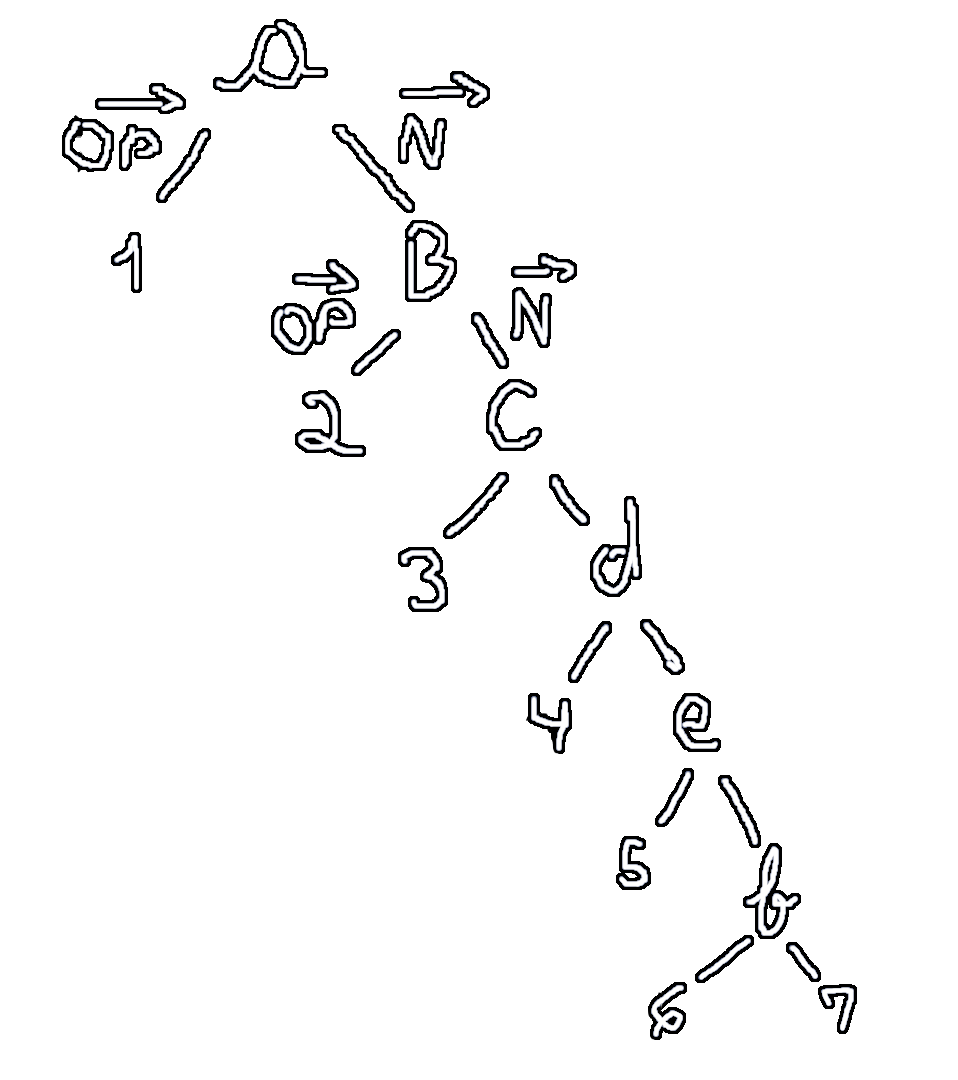
\includegraphics{q7.png}
		\end{minipage}
	\end{enumerate}
